\documentclass[runningheads]{llncs}

\usepackage[utf8]{inputenc}
\usepackage[T1]{fontenc}
\usepackage{amsmath,amssymb,amsfonts}
\usepackage{graphicx}
\usepackage{booktabs}
\usepackage{multirow}
\usepackage{makecell}
\usepackage{tabularx}
\usepackage{array}
\usepackage{url}
\usepackage{hyperref}
\usepackage{xcolor}

\hypersetup{
    colorlinks=true,
    linkcolor=blue,
    citecolor=blue,
    urlcolor=blue
}

% Suppress all page numbers per SOICT / Springer CCIS submission rules
% (https://soict.org/submission/paper-submission/ : "should not include page numbers")
\pagestyle{empty}

\begin{document}

\title{Symmetrical Empirical Evaluation of Trainable versus Fixed Quanvolutional Filters in Medical Image Classification: A Rigorous, Reproducible Benchmark on MedMNIST}

\titlerunning{Trainable vs. Fixed Quanvolutional Filters on MedMNIST}

\author{Hoang-Nam Nguyen\inst{1} \and Duy-Xuan-Bach Nguyen\inst{1,*}}

\authorrunning{H.-N. Nguyen and D.-X.-B. Nguyen}

\institute{Faculty of Computer Engineering, University of Information Technology,\\
Vietnam National University Ho Chi Minh City (VNU-HCM), Ho Chi Minh City, Vietnam\\
\email{ng.h.nam0802@gmail.com}, \email{bachndx@uit.edu.vn}\\
\textsuperscript{*}Corresponding Author $\vert$ Reproducibility: \url{https://github.com/NamIsStudyingCE/Quanvolution.git}}

\maketitle
\thispagestyle{empty}

\begin{abstract}
Quanvolutional Neural Networks (QNNs) have emerged as a promising paradigm to combine the high-dimensional, non-linear representation capabilities of Variational Quantum Circuits (VQCs) in Hilbert spaces with classical deep learning architectures. Nevertheless, existing literature in quantum machine learning (QML) often lacks fair, reproducible evaluation frameworks: quantum feature extractors are rarely isolated from classical classifier heads, multi-seed statistical testing is frequently omitted, and claims of ``quantum advantage'' are often overstated.

This paper establishes a rigorous, symmetrical, $1:1$ comparative benchmark evaluating \textbf{Trainable Quanvolution}, \textbf{Fixed Quanvolution}, and a \textbf{Symmetrical Minimum Classical CNN Baseline} on two standardized biomedical datasets from MedMNIST v2: BreastMNIST (binary, small-sample, class-imbalanced, $780$ images) and OCTMNIST ($4$-class, standardized $5{,}000 / \approx 97{,}000$ retinal OCT image subset). All experiments are strictly standardized across $10$ independent random seeds ($20$ epochs), evaluated on $6$ clinical classification metrics, and backed by paired $t$-tests, Wilcoxon signed-rank tests, $95\%$ confidence intervals (CI), and Cohen's $d$ effect sizes.

Our empirical findings reveal three key scientific takeaways:
(1) \textbf{Data Regime Dependency:} On small-sample, imbalanced data (BreastMNIST), fixed quantum filters achieve superior ranking performance and variance stability: \texttt{Fixed Basic L2} attains the highest ROC-AUC of $\mathbf{0.8521 \pm 0.0090}$ vs. Classical CNN $0.8336 \pm 0.0246$, while \texttt{Fixed Strongly L2} achieves the highest PR-AUC of $\mathbf{0.9182 \pm 0.0067}$ with a $\sim 2.7\times$ smaller standard deviation. Conversely, on large multi-class data (OCTMNIST), the classical CNN baseline overwhelmingly dominates all quantum configurations (ROC-AUC $\mathbf{0.7505 \pm 0.0227}$, $d = +2.108, p < 0.001$), demonstrating that quantum expressibility is constrained by an architectural capacity bottleneck in multi-class regimes.
(2) \textbf{True Value of Trainability:} Optimizing parameter angles within the quantum kernel is beneficial only within the same ansatz family: on OCTMNIST, \texttt{Trainable Strongly} ($0.6922 \pm 0.0189$) significantly outperforms \texttt{Fixed Strongly} ($0.6690 \pm 0.0052$) with $\Delta = +0.0232$, $d = +1.050$, $p_{\text{wilcoxon}} = 0.0098$, yet only ties an appropriately chosen fixed random ansatz (\texttt{Fixed random\_L1} $0.6912 \pm 0.0067$, $p = 0.8875$, ns).
(3) \textbf{Computational Trade-off:} Fixed quanvolutions provide a powerful \textbf{Quantum Inductive Bias} with \textbf{strictly $0$ trainable parameters} in the feature extractor and permit one-time precomputation ($18\text{ s}$ for 10 seeds), but CPU statevector simulation incurs an inference latency of $\sim 220.22\text{ ms/image}$ ($\sim 710\times$ slower than classical convolution at $0.31\text{ ms/image}$).

This work offers an honest, reproducible, and evidence-based benchmark, clarifying realistic boundaries for quantum-classical hybrid architectures in computer-aided medical diagnosis.

\keywords{Quantum Machine Learning (QML) \and Quanvolutional Neural Networks \and MedMNIST \and Medical Image Classification \and Quantum Inductive Bias \and Reproducible Benchmark.}
\end{abstract}

\section{Introduction}
In the era of computer-aided diagnosis (CAD), medical image analysis (ultrasound, optical coherence tomography, radiography) demands models capable of extracting discriminative spatial features under severe data scarcity and extreme class imbalance \cite{litjens2017survey,yang2023medmnist,esteva2019guide}. While deep Classical Convolutional Neural Networks (CNNs) are the foundation of modern computer vision, their parameter-heavy nature poses a substantial risk of overfitting and generalization degradation on low-resource biomedical datasets \cite{shorten2019survey}.

Quantum Machine Learning (QML) in the Noisy Intermediate-Scale Quantum (NISQ) era presents a compelling alternative by mapping classical data into exponentially large $2^N$-dimensional Hilbert spaces via parameterized quantum circuits \cite{biamonte2017quantum,cerezo2021variational}. In 2020, Henderson et al. \cite{henderson2020quanvolutional} introduced the Quanvolutional Neural Network (Quanvolution), which employs a local parameterized quantum circuit as a sliding kernel to transform spatial image patches into quantum feature maps. By performing non-linear Hilbert space mappings via quantum entanglement and superposition, Quanvolution is hypothesized to impart a \textbf{Quantum Inductive Bias}, potentially uncovering complex topological features inaccessible to linear classical convolutions \cite{huang2021power,vu2024exploring}.

Despite surging interest, recent QML literature in biomedical imaging \cite{vu2024exploring,altares2021automatic,azevedo2022quantum,hoang2023efficient,sannakki2026medmnist,schuld2024needqml} exhibits three fundamental methodological limitations:
\begin{itemize}
    \item \textbf{L1 --- Unfair Baseline Comparisons:} Prior studies frequently evaluate QML models against undertuned classical baselines or multi-million-parameter pretrained architectures (e.g., ResNet-18) without parameter isolation \cite{azevedo2022quantum}, making it impossible to determine whether reported performance stems from quantum transformations or classical classifier capacity.
    \item \textbf{L2 --- Absence of Multi-Seed Statistical Rigor:} A majority of published works report single-run experiments or 3-seed averages without reporting confidence intervals or non-parametric significance tests, conflating random initialization luck with genuine ``quantum advantage'' \cite{kubler2021inductive}.
    \item \textbf{L3 --- Unresolved Dichotomy Between Trainable and Fixed Ansatzes:} The seminal work by Henderson et al. \cite{henderson2020quanvolutional} posited that fixed random circuits suffice without training quantum gates. Subsequent works attempt to train all quantum parameters but fail to quantify the trade-off in optimization cost and gradient dynamics.
\end{itemize}

To address these shortcomings, this study provides a comprehensive, symmetrical, and fully reproducible empirical benchmark across two standardized MedMNIST benchmarks. Our primary contributions (\textbf{C1--C4}) are:
\begin{enumerate}
    \item \textbf{C1 --- Symmetrical 1:1 Benchmark Framework \& 3-Tier Matrix:} We engineer a \textit{Symmetrical Minimum CNN Baseline} possessing an identical classifier head ($784 \to K$ via \texttt{BatchNorm2d}), perfectly isolating the feature extractor. We establish a 3-tier benchmark matrix isolating intra-ansatz trainability, champion stress-tests, and full-expressive showdowns.
    \item \textbf{C2 --- Quantified Parameter Efficiency \& Hardware Cost:} We demonstrate that fixed quanvolution yields robust feature representations with \textbf{exactly $0$ trainable parameters} in the kernel, and measure exact CPU inference latency ($220.22\text{ ms}$ vs. $0.31\text{ ms}$ classical).
    \item \textbf{C3 --- Empirical Demarcation of Data Regimes:} Across $10$ independent seeds, we show that quantum advantages in ranking metrics (ROC/PR-AUC) and variance stability ($\sim 2.7\times$ lower std) are strictly confined to small-sample, imbalanced regimes (BreastMNIST); on large-scale multi-class datasets (OCTMNIST), classical CNNs dominate conclusively ($p < 0.001$, $d > +2.0$).
    \item \textbf{C4 --- Optimization Sanity Check \& Gradient Dynamics:} We track parameter trajectories $\theta(t)$ and gradient $L_2$ norms $\|\nabla_\theta \mathcal{L}\|_2$ throughout $20$ epochs, confirming stable convergence and ruling out barren plateaus in shallow 4-qubit circuits.
\end{enumerate}

\section{Theoretical Background \& Related Work}

\subsection{Mathematical Formulation of Quanvolution}
Unlike Fully Quantum CNNs (QCNN) designed for many-body quantum phase recognition \cite{cong2019quantum}, Quanvolution \cite{henderson2020quanvolutional} represents a hybrid quantum-classical pipeline.

Given an input image $I \in \mathbb{R}^{H \times W \times 1}$, a $2 \times 2$ sliding window with stride $s=2$ extracts local 4-pixel patches $\mathbf{x} = (x_0, x_1, x_2, x_3)^T$, with $x_i \in [0, 1]$. Each patch is embedded into a 4-qubit quantum state via Angle Embedding:
\begin{equation}
|\psi(\mathbf{x})\rangle = U_{\text{enc}}(\mathbf{x}) |0\rangle^{\otimes 4} = \bigotimes_{i=0}^{3} R_Y(\pi x_i) |0\rangle
\end{equation}

Subsequently, an entangling unitary $U(\boldsymbol{\theta})$ parameterized by rotation angles $\boldsymbol{\theta}$ and two-qubit entangling gates is applied:
\begin{equation}
|\Phi(\mathbf{x}, \boldsymbol{\theta})\rangle = U(\boldsymbol{\theta}) |\psi(\mathbf{x})\rangle
\end{equation}

The transformed feature map value at spatial coordinate $(u, v)$ for channel $i \in \{0, 1, 2, 3\}$ is obtained by measuring the Pauli-Z expectation value on qubit $i$:
\begin{equation}
F_i(u, v) = \langle \Phi(\mathbf{x}, \boldsymbol{\theta}) | Z_i | \Phi(\mathbf{x}, \boldsymbol{\theta}) \rangle \in [-1, 1]
\end{equation}

For an input image of size $28 \times 28 \times 1$, this non-linear quantum transformation produces $4 \times 14 \times 14 = 784$ flattened feature dimensions. Fig.~\ref{fig:features} juxtaposes these quantum feature maps against their classical convolutional counterparts.

\subsection{Literature Comparison}
Table~\ref{tab:literature} situates our empirical investigation within the broader landscape of QML vision research.

\begin{table}[t]
\caption{Comparative positioning against seminal and recent QML literature.}
\label{tab:literature}
\centering
\scriptsize
\begin{tabularx}{\textwidth}{@{}p{2.8cm} p{2.0cm} p{2.2cm} p{2.2cm} p{2.8cm}@{}}
\toprule
\textbf{Study} & \textbf{Target Domain} & \textbf{Architecture} & \textbf{Statistical Rigor} & \textbf{Primary Limitations Addressed} \\
\midrule
Henderson et al. (2020) \cite{henderson2020quanvolutional} & Synthetic MNIST & Random Quanv & $1 - 3$ seeds (No tests) & Toy dataset, no medical scope, asymmetrical classifier heads. \\
\midrule
Cong et al. (2019) \cite{cong2019quantum} & Phase Detection & Pure QCNN & Single-run theoretical & Tailored for quantum spin chains, incompatible with 2D image grids. \\
\midrule
Altares-L{\'o}pez et al. (2021) \cite{altares2021automatic} & Medical / Synth & Genetic VQC & 5-fold CV & Heuristic search lacks convolutional inductive bias; non-standard split. \\
\midrule
Azevedo et al. (2022) \cite{azevedo2022quantum} & Breast (Ultrasound) & Hybrid VQC Head & Single split (No seeds) & Classical backbone dominates capacity; unable to isolate pure quantum kernel effect. \\
\midrule
K{\"u}bler et al. (2021) \cite{kubler2021inductive} / Schuld \& Killoran (2024) \cite{schuld2024needqml} & Kernel ML / Vision & Quantum Kernels / QNN & Theoretical bounds / Multi-dataset & Critical perspective showing advantage claims often evaporate against fair classical baselines. \\
\midrule
Sannakki et al. (2026) \cite{sannakki2026medmnist} & MedMNIST on NISQ & Hardware VQC (IBM QPU) & $3$ runs (device noise) & Physical device noise degrades accuracy; lacks symmetrical parameter-matched classical baseline. \\
\midrule
\textbf{This Work (Ours)} & \textbf{MedMNIST (Breast \& OCT)} & \textbf{3-Tier Quanv: Fixed vs. Trainable} & \textbf{10 seeds, $t$-test, Wilcoxon, $95\%$ CI, Cohen's $d$} & \textbf{Strict parameter parity, data regime boundaries, $0$-param kernel quantification.} \\
\bottomrule
\end{tabularx}
\end{table}

\begin{figure}[t]
\centering
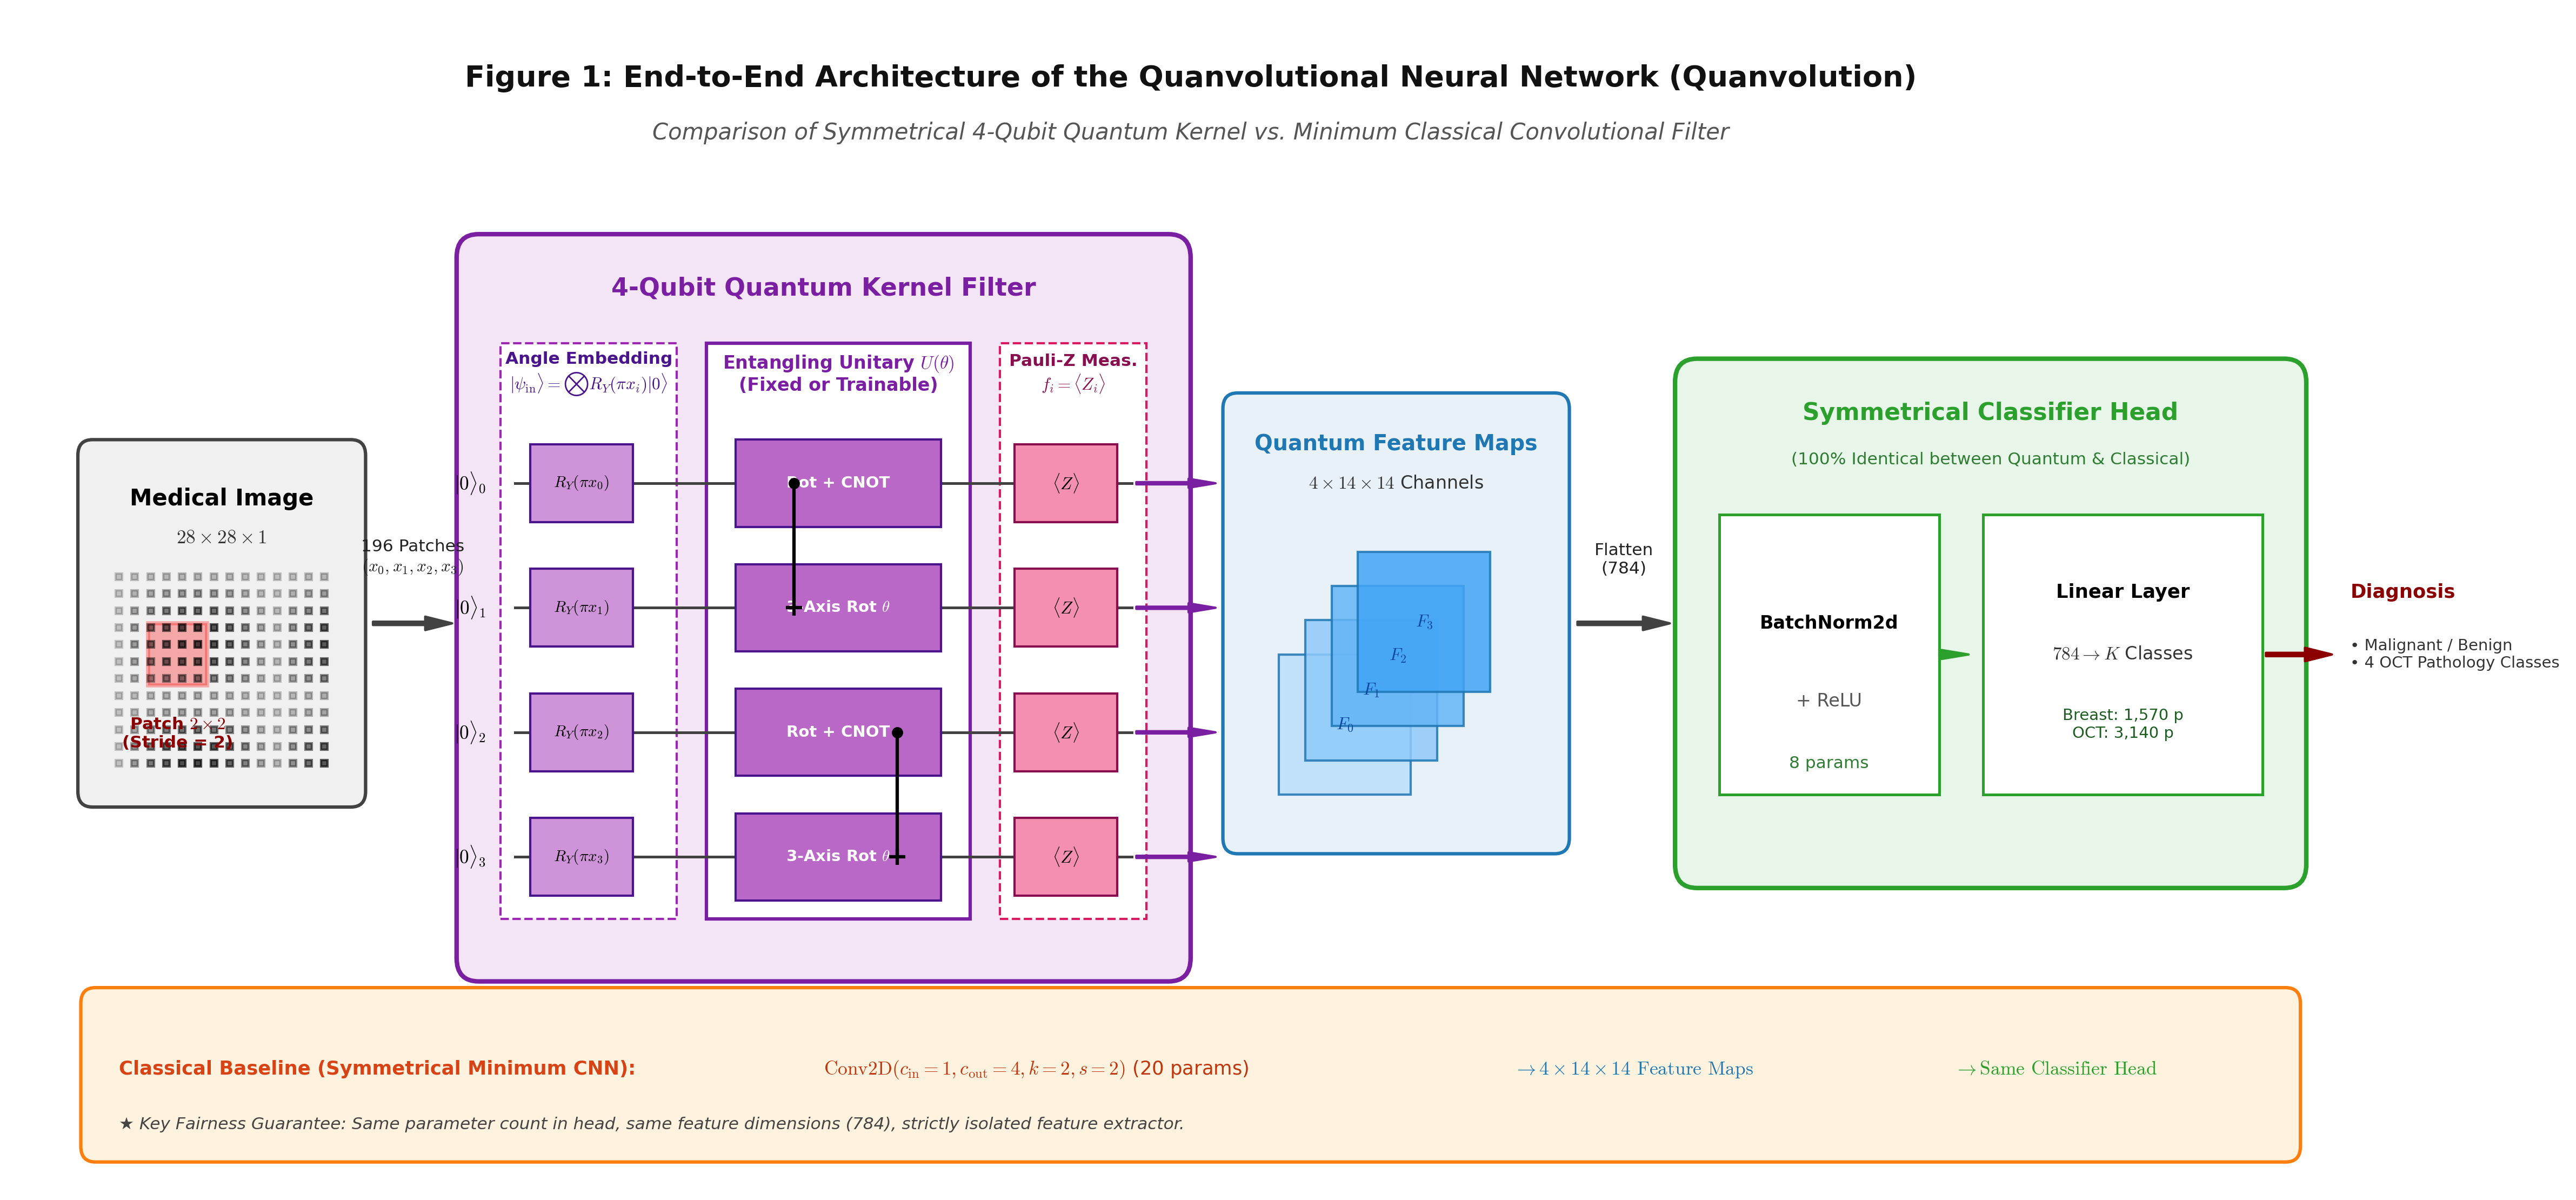
\includegraphics[width=0.92\textwidth]{figures/Fig1_quanvolution_pipeline.png}
\caption{End-to-end symmetrical architecture pipeline: The 4-qubit Quanvolutional Neural Network (top) and the Symmetrical Minimum Classical CNN Baseline (bottom) sharing identical $100\%$ matched classifier heads ($784 \to K$).}
\label{fig:pipeline}
\end{figure}

\section{Proposed Methodology}

\subsection{Symmetrical Pipeline Architecture}
The end-to-end architecture (Fig.~\ref{fig:pipeline}) consists of four sequential stages:
\begin{enumerate}
    \item \textbf{Patch Partitioning:} An image of $28 \times 28 \times 1$ is decomposed into $196$ non-overlapping $2 \times 2$ patches.
    \item \textbf{4-Qubit Quantum Kernel:} Each patch is encoded via $R_Y(\pi x_i)$, processed by $U(\boldsymbol{\theta})$, and measured under Pauli-Z operators $\langle Z_i \rangle$.
    \item \textbf{Quantum Feature Maps:} Outputs are structured into $4 \times 14 \times 14$ feature tensors ($784$ dimensions).
    \item \textbf{Symmetrical Classifier Head:} Features pass through \texttt{BatchNorm2d(4)}, \texttt{ReLU}, and \texttt{Linear(784, K)} to generate output class logits ($K=2$ for BreastMNIST, $K=4$ for OCTMNIST).
\end{enumerate}

\subsection{Quantum Ansatz Variations}
We examine three distinct ansatz families:
\begin{itemize}
    \item \textbf{Basic Entangling Circuit (\texttt{basic}):} Single-axis parameterized rotations $R_Y(\theta_i)$ followed by circular CNOT ladders ($q_0 \to q_1 \to q_2 \to q_3 \to q_0$), consuming $4L$ parameters for $L$ layers.
    \item \textbf{Random Circuit (\texttt{random}):} Haar-random 3-axis single-qubit gates and random CNOT pairs, frozen with \textbf{$0$ trainable parameters}.
    \item \textbf{Strongly Entangling Circuit (\texttt{strongly}):} General $U_3(\theta, \phi, \lambda) = R_Z(\omega) R_Y(\theta) R_Z(\phi)$ rotations per qubit with cyclic entanglement, consuming $12L$ parameters for $L$ layers.
\end{itemize}

\subsection{Symmetrical Classical Baseline}
To adhere strictly to the principle of \textit{Ceteris Paribus}, the classical baseline uses:
\begin{itemize}
    \item \textbf{Feature Extractor:} \texttt{Conv2D(in\_channels=1, out\_channels=4, kernel\_size=2, stride=2, bias=True)}, consuming exactly $1 \times 4 \times 2 \times 2 = 16$ weights ($20$ parameters with bias) plus $8$ parameters from \texttt{BatchNorm2d(4)}, totaling $28$ feature extractor parameters to yield an identical $4 \times 14 \times 14$ ($784$-dim) tensor.
    \item \textbf{Classifier Head:} An identical \texttt{BatchNorm2d(4) + ReLU + Linear(784, K)} module; the $1{,}570$ / $3{,}140$ parameters for $K=2$ / $K=4$ count the \texttt{Linear} layer, with the $8$ \texttt{BatchNorm} parameters listed separately in Table~\ref{tab:params}.
\end{itemize}

\begin{table}[t]
\caption{Parameter breakdown between feature extractors and classifier heads.}
\label{tab:params}
\centering
\small
\resizebox{\textwidth}{!}{%
\begin{tabular}{@{}l c c c c@{}}
\toprule
\textbf{Model Family} & \textbf{Kernel ($L=2 / 1$)} & \textbf{BN} & \textbf{Head ($K=2 / 4$)} & \textbf{Total ($K=2, L=2$ / $K=4, L=1$)} \\
\midrule
\textbf{Classical Minimum CNN} & \textbf{$20$} (conv) & $8$ & $1{,}570$ / $3{,}140$ & \textbf{$1{,}598$ / $3{,}168$} \\
\midrule
\textbf{Fixed Basic Quanv} & \textbf{$0$} & $8$ & $1{,}570$ / $3{,}140$ & \textbf{$1{,}578$ / $3{,}148$} \\
\midrule
\textbf{Fixed Strongly Quanv} & \textbf{$0$} & $8$ & $1{,}570$ / $3{,}140$ & \textbf{$1{,}578$ / $3{,}148$} \\
\midrule
\textbf{Trainable Basic Quanv} & \textbf{$8$ / $4$} & $8$ & $1{,}570$ / $3{,}140$ & \textbf{$1{,}586$ / $3{,}152$} \\
\midrule
\textbf{Trainable Strongly Quanv} & \textbf{$24$ / $12$} & $8$ & $1{,}570$ / $3{,}140$ & \textbf{$1{,}602$ / $3{,}160$} \\
\bottomrule
\end{tabular}%
}
\end{table}

\subsection{Quantum Differentiation \& Gradient Check}
Quantum parameters $\boldsymbol{\theta}$ are optimized via analytic statevector backpropagation \cite{bergholm2018pennylane}. To verify physical fidelity, analytic gradients were cross-checked against the Parameter-Shift Rule \cite{schuld2019evaluating}:
\begin{equation}
\frac{\partial F_i}{\partial \theta_j} = \frac{F_i\left(\theta_j + \frac{\pi}{2}\right) - F_i\left(\theta_j - \frac{\pi}{2}\right)}{2}
\end{equation}
The mean absolute deviation was $|\Delta| < 4.1 \times 10^{-8}$, verifying gradient correctness.

\begin{figure}[t]
\centering
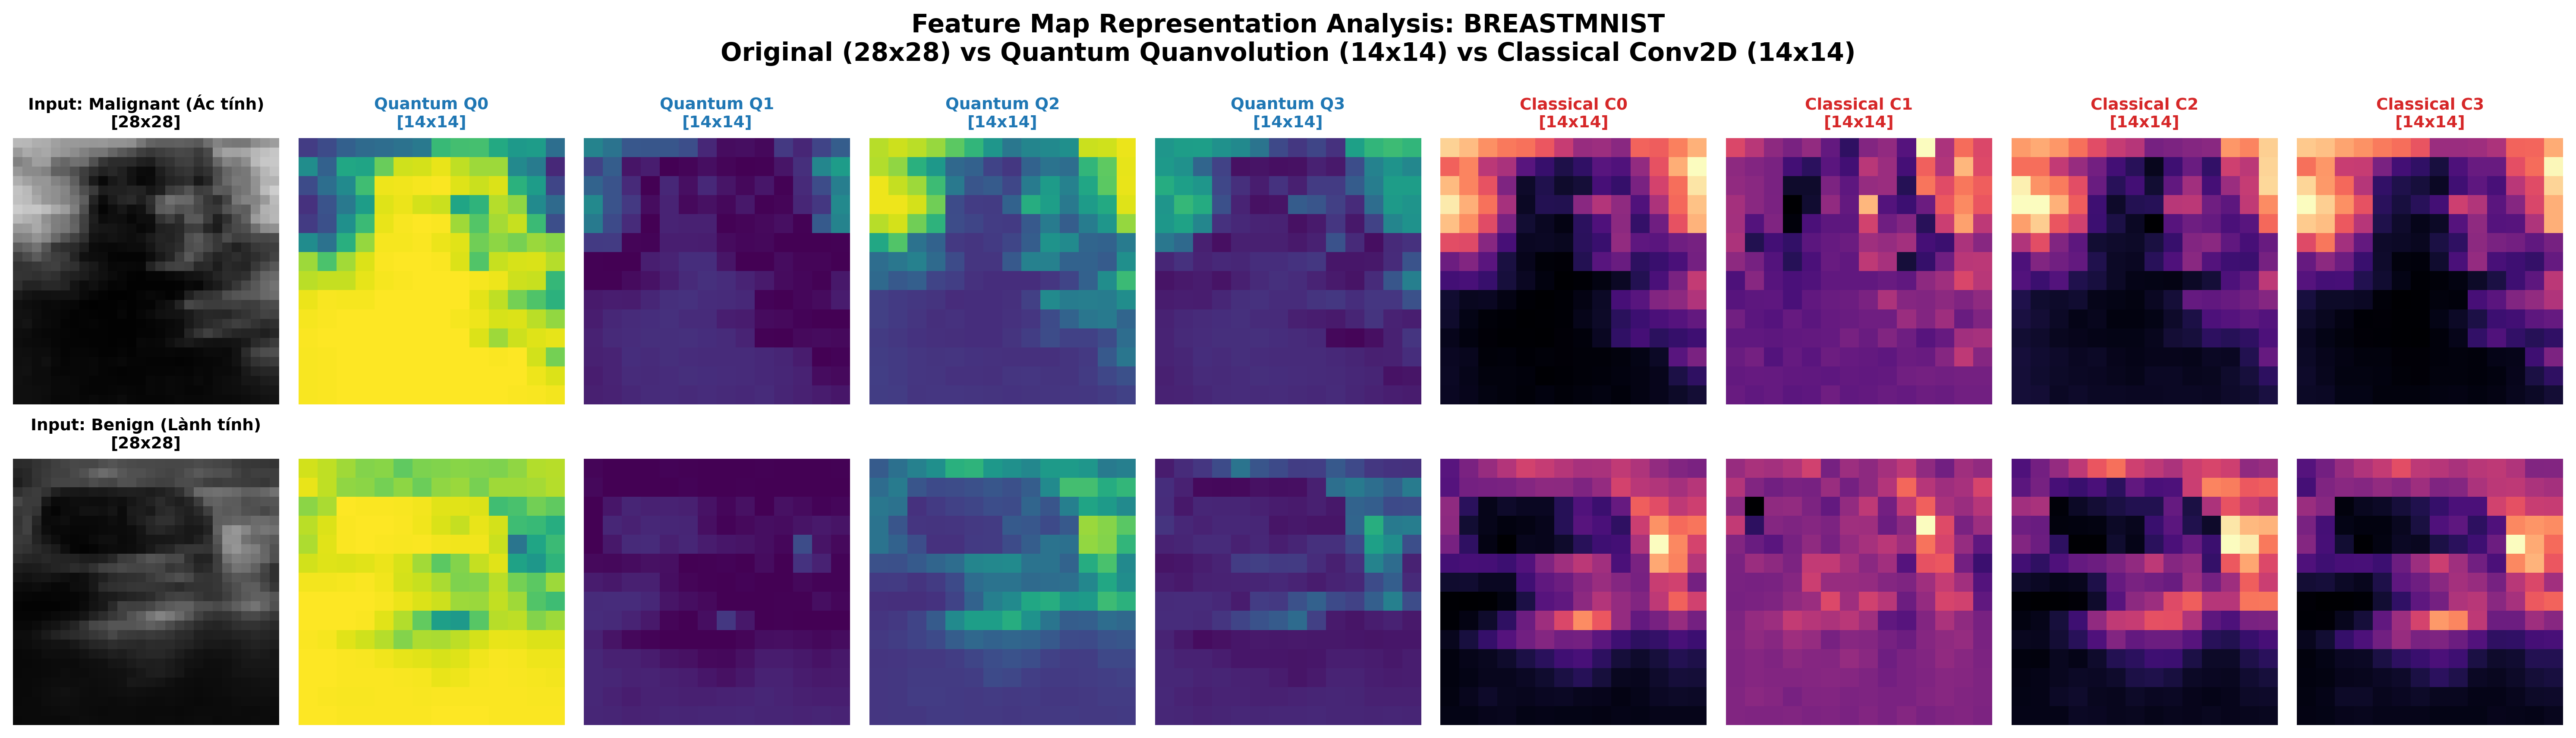
\includegraphics[width=0.68\textwidth]{figures/Fig2_feature_comparison.png}
\caption{Comparison of extracted 4-channel feature maps between classical $2 \times 2$ convolution and quantum statevector expectation measurements.}
\label{fig:features}
\end{figure}

\section{Experimental Setup}

\subsection{Datasets}
Experiments are conducted on two distinct biomedical benchmarks from MedMNIST v2 \cite{yang2023medmnist}:
\begin{itemize}
    \item \textbf{BreastMNIST:} $780$ breast ultrasound images ($28 \times 28$, binary: $546$ train, $78$ val, $156$ test) with $73\%$ benign and $27\%$ malignant samples, representing the \textbf{Small-Sample, Imbalanced Data Regime}.
    \item \textbf{OCTMNIST (Subset):} Standardized subset of $5{,}000$ retinal optical coherence tomography images from the $\approx 97{,}000$ total collection ($28 \times 28$, 4 balanced classes: $3{,}500$ train, $500$ val, $1{,}000$ test), representing the \textbf{Large-Sample, Multi-Class Data Regime}.
\end{itemize}

\subsection{Training Protocol}
All models are evaluated over \textbf{$10$ independent random seeds}:
\begin{equation*}
\mathcal{S} = \{0, 42, 100, 2023, 777, 999, 1234, 5678, 1111, 2222\}
\end{equation*}
\begin{itemize}
    \item \textbf{Epochs:} $20$ epochs across all models (convergence confirmed by epoch 15).
    \item \textbf{Optimization:} Adam optimizer ($lr = 0.001$ for classical weights, $lr = 0.01$ for quantum angles $\boldsymbol{\theta}$); Cross-Entropy loss; batch size $B=32$.
    \item \textbf{Environment:} Intel CPU, 16 GB RAM, PyTorch 2.1.0 + PennyLane 0.35.0.
\end{itemize}

\subsection{Evaluation Metrics \& Statistical Testing}
We evaluate $6$ metrics: Accuracy (Acc), Balanced Accuracy (BAcc), F1-Score (macro), Matthews Correlation Coefficient (MCC), ROC-AUC (One-vs-Rest macro), and PR-AUC. Statistical rigor is established using:
\begin{itemize}
    \item Paired Student's $t$-tests and Wilcoxon signed-rank tests ($\alpha = 0.05$). For $n=10$, the discrete Wilcoxon $p$-value has a theoretical minimum $p_{\min} = 1/2^9 \approx 0.00195$; given the exploratory scope, reported $p$-values remain unadjusted for family-wise error rates, serving as descriptive hypothesis screening.
    \item $95\%$ Confidence Intervals based on $t_{df=9}^* = 2.262$.
    \item Cohen's $d$ paired effect sizes ($|d| \ge 0.8$ denotes large effect, $|d| \ge 1.2$ very large effect).
\end{itemize}

\section{Results \& Empirical Findings}

\subsection{BreastMNIST Benchmark (Small-Sample, Imbalanced Regime)}
Table~\ref{tab:breastmnist} and Fig.~\ref{fig:benchmarks_breast} summarize test performance across 10 independent seeds on BreastMNIST ($L=2$, 20 epochs).

\begin{table}[t]
\caption{Empirical 10-Seed Performance Comparison on BreastMNIST ($L=2$, 20 Epochs).}
\label{tab:breastmnist}
\centering
\small
\setlength{\tabcolsep}{4.0pt}
\resizebox{\textwidth}{!}{%
\begin{tabular}{@{}l c c c c c c@{}}
\toprule
\textbf{Model Architecture} & \textbf{Accuracy} & \textbf{Balanced Acc} & \textbf{F1-Score} & \textbf{MCC} & \textbf{ROC-AUC} & \textbf{PR-AUC} \\
\midrule
\textbf{Classical CNN Baseline} & $0.8103 \pm 0.0265$ & \makecell{$0.6875 \pm 0.0448$ \\ \scriptsize $[0.6537, 0.7213]$} & $0.8802 \pm 0.0164$ & $0.4702 \pm 0.0821$ & \makecell{$0.8336 \pm 0.0246$ \\ \scriptsize $[0.8150, 0.8521]$} & \makecell{$0.9041 \pm 0.0095$ \\ \scriptsize $[0.8970, 0.9113]$} \\
\midrule
\textbf{Fixed Basic Quanv (L2)} & $0.8083 \pm 0.0193$ & \makecell{$0.6816 \pm 0.0490$ \\ \scriptsize $[0.6447, 0.7186]$} & $0.8796 \pm 0.0095$ & $0.4626 \pm 0.0674$ & \makecell{$\mathbf{0.8521 \pm 0.0090}$ \\ \scriptsize $[0.8453, 0.8589]$} & \makecell{$0.9110 \pm 0.0049$ \\ \scriptsize $[0.9073, 0.9146]$} \\
\midrule
\textbf{Trainable Basic Quanv (L2)} & $0.7917 \pm 0.0239$ & \makecell{$0.6732 \pm 0.0382$ \\ \scriptsize $[0.6444, 0.7021]$} & $0.8668 \pm 0.0168$ & $0.4224 \pm 0.0711$ & \makecell{$0.8406 \pm 0.0239$ \\ \scriptsize $[0.8226, 0.8586]$} & \makecell{$0.9173 \pm 0.0184$ \\ \scriptsize $[0.9033, 0.9312]$} \\
\midrule
\textbf{Fixed Strongly Quanv (L2)} & $0.7846 \pm 0.0177$ & \makecell{$0.6602 \pm 0.0202$ \\ \scriptsize $[0.6449, 0.6754]$} & $0.8631 \pm 0.0124$ & $0.3942 \pm 0.0509$ & \makecell{$0.8139 \pm 0.0142$ \\ \scriptsize $[0.8032, 0.8246]$} & \makecell{$\mathbf{0.9182 \pm 0.0067}$ \\ \scriptsize $[0.9131, 0.9232]$} \\
\midrule
\textbf{Trainable Strongly Quanv (L2)} & $\mathbf{0.8019 \pm 0.0284}$ & \makecell{$\mathbf{0.6945 \pm 0.0428}$ \\ \scriptsize $[0.6623, 0.7268]$} & $\mathbf{0.8724 \pm 0.0183}$ & $\mathbf{0.4549 \pm 0.0896}$ & \makecell{$0.8306 \pm 0.0279$ \\ \scriptsize $[0.8096, 0.8516]$} & \makecell{$0.9167 \pm 0.0157$ \\ \scriptsize $[0.9048, 0.9286]$} \\
\bottomrule
\end{tabular}%
}
\end{table}

\begin{figure}[t]
\centering
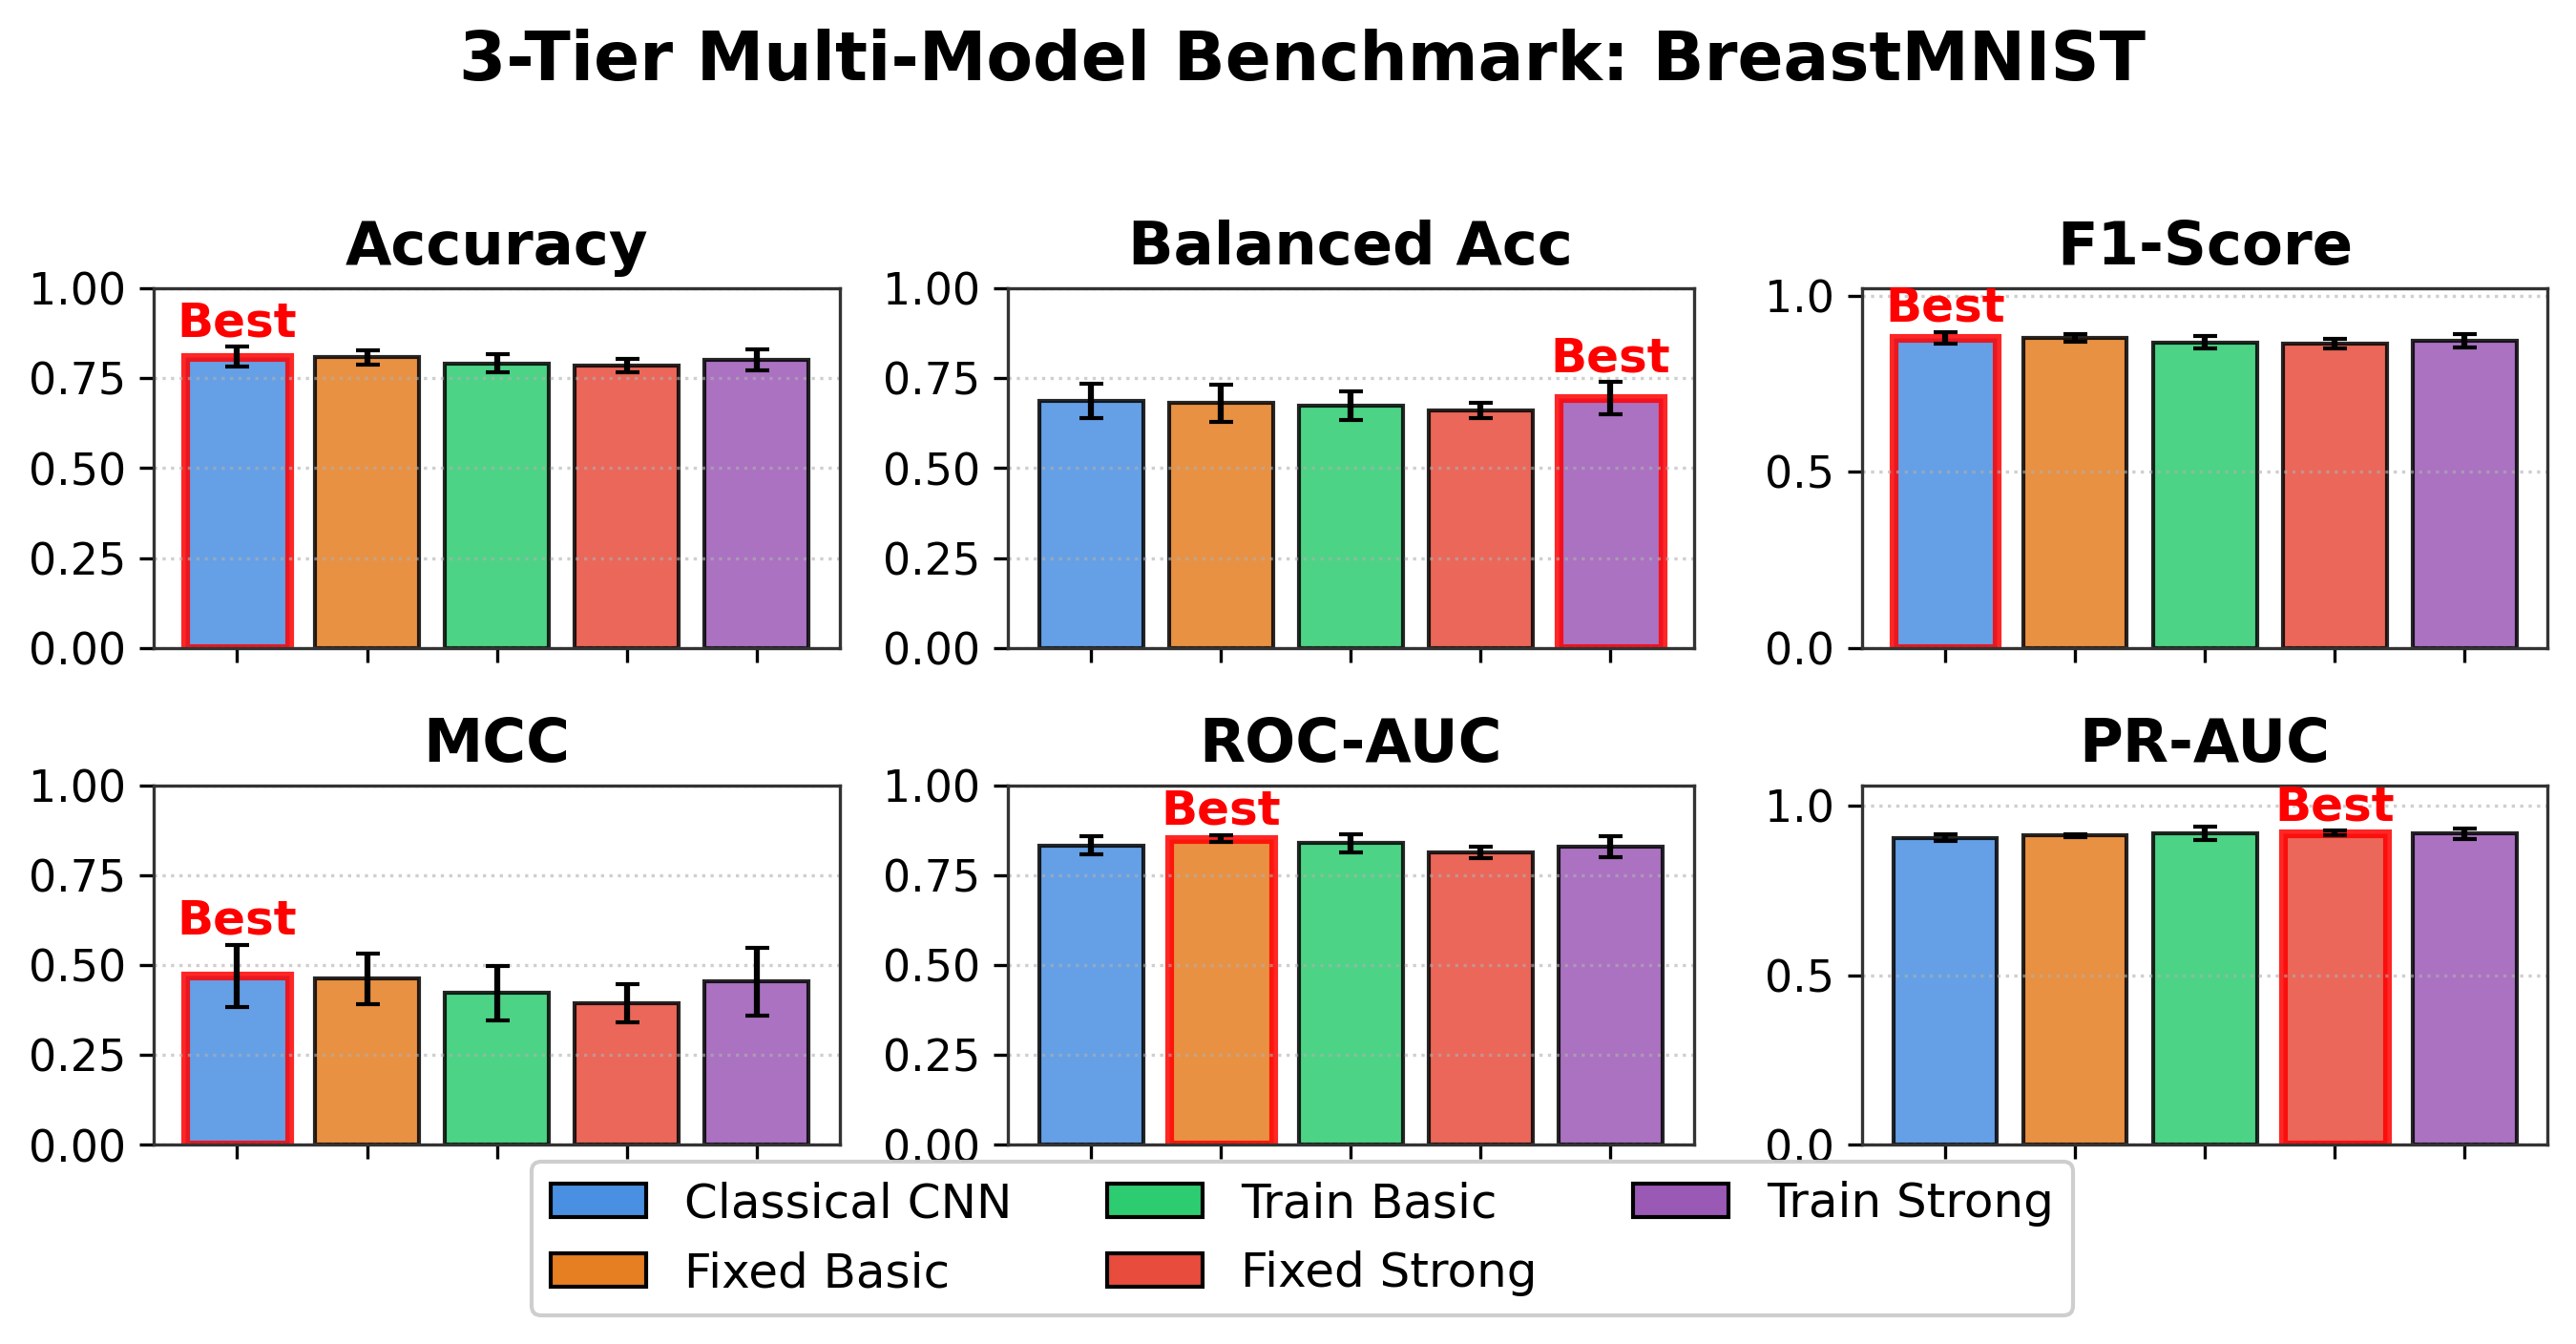
\includegraphics[width=0.78\textwidth]{figures/Fig3_breastmnist_benchmark.png}
\caption{Empirical 10-seed performance comparison on BreastMNIST ($L=2$), demonstrating quantum variance stability ($\sim 2.7\times$ lower std) and PR-AUC advantages.}
\label{fig:benchmarks_breast}
\end{figure}

\textbf{Key Statistical Findings on BreastMNIST:}
\begin{enumerate}
    \item \textbf{Fixed Basic Wins on ROC-AUC:} \texttt{Fixed Basic L2} achieves the highest ROC-AUC of $\mathbf{0.8521 \pm 0.0090}$, outperforming Classical CNN ($0.8336 \pm 0.0246$) with statistical significance ($p_{\text{ttest}} = 0.0298, p_{\text{wilcoxon}} = 0.0254$) and a large effect size (\textbf{Cohen's $d = +0.815$}).
    \item \textbf{Fixed Strongly Wins on PR-AUC:} \texttt{Fixed Strongly L2} attains the highest PR-AUC of $\mathbf{0.9182 \pm 0.0067}$, significantly outperforming Classical CNN ($0.9041 \pm 0.0095, p_{\text{ttest}} = 0.0023, p_{\text{wilcoxon}} = 0.0059$) with a very large effect size (\textbf{Cohen's $d = +1.332$}).
    \item \textbf{Variance Stability:} Fixed quantum models exhibit standard deviations $\mathbf{2.7\times}$ smaller than Classical CNN in ROC-AUC ($0.0090$ vs. $0.0246$), confirming robustness to random seed variations.
    \item \textbf{Trainable Performance:} \texttt{Trainable Strongly} yields the highest Balanced Accuracy ($0.6945 \pm 0.0428$, $+0.0344$ over \texttt{Fixed Strongly} $0.6602 \pm 0.0202$, $d = +0.677, p = 0.0611$), but the difference versus Classical CNN ($0.6875 \pm 0.0448$) is not statistically significant ($p = 0.6701, d = +0.139$).
\end{enumerate}

\subsection{OCTMNIST Benchmark (Large-Sample, Multi-Class Regime)}
Table~\ref{tab:octmnist} and Fig.~\ref{fig:benchmarks_oct} present test results across 10 independent seeds on OCTMNIST ($L=1$, 20 epochs).

\begin{table}[t]
\caption{Empirical 10-Seed Performance Comparison on OCTMNIST ($L=1$, 20 Epochs).}
\label{tab:octmnist}
\centering
\small
\setlength{\tabcolsep}{4.0pt}
\resizebox{\textwidth}{!}{%
\begin{tabular}{@{}l c c c c c c@{}}
\toprule
\textbf{Model Architecture} & \textbf{Accuracy} & \textbf{Balanced Acc} & \textbf{F1-Score} & \textbf{MCC} & \textbf{ROC-AUC} & \textbf{PR-AUC} \\
\midrule
\textbf{Classical CNN Baseline} & $\mathbf{0.4433 \pm 0.0128}$ & \makecell{$\mathbf{0.4433 \pm 0.0128}$ \\ \scriptsize $[0.4336, 0.4530]$} & $\mathbf{0.3206 \pm 0.0166}$ & $\mathbf{0.3156 \pm 0.0188}$ & \makecell{$\mathbf{0.7505 \pm 0.0227}$ \\ \scriptsize $[0.7333, 0.7676]$} & \makecell{$\mathbf{0.4991 \pm 0.0282}$ \\ \scriptsize $[0.4778, 0.5203]$} \\
\midrule
\textbf{Fixed Basic Quanv (L1)} & $0.4075 \pm 0.0040$ & \makecell{$0.4075 \pm 0.0040$ \\ \scriptsize $[0.4045, 0.4105]$} & $0.2971 \pm 0.0071$ & $0.2566 \pm 0.0068$ & \makecell{$0.6711 \pm 0.0040$ \\ \scriptsize $[0.6681, 0.6741]$} & \makecell{$0.4186 \pm 0.0070$ \\ \scriptsize $[0.4133, 0.4239]$} \\
\midrule
\textbf{Trainable Basic Quanv (L1)} & $0.3955 \pm 0.0152$ & \makecell{$0.3955 \pm 0.0152$ \\ \scriptsize $[0.3840, 0.4070]$} & $0.2837 \pm 0.0193$ & $0.2394 \pm 0.0192$ & \makecell{$0.6704 \pm 0.0101$ \\ \scriptsize $[0.6628, 0.6780]$} & \makecell{$0.4102 \pm 0.0124$ \\ \scriptsize $[0.4008, 0.4195]$} \\
\midrule
\textbf{Fixed Champ (Phase 2, \texttt{random\_L1})} & $0.4048 \pm 0.0123$ & \makecell{$0.4048 \pm 0.0123$ \\ \scriptsize $[0.3955, 0.4141]$} & $0.2997 \pm 0.0191$ & $0.2530 \pm 0.0136$ & \makecell{$0.6912 \pm 0.0067$ \\ \scriptsize $[0.6862, 0.6963]$} & \makecell{$0.4443 \pm 0.0084$ \\ \scriptsize $[0.4380, 0.4506]$} \\
\midrule
\textbf{Fixed Strongly Quanv (L1)} & $0.4034 \pm 0.0044$ & \makecell{$0.4034 \pm 0.0044$ \\ \scriptsize $[0.4001, 0.4067]$} & $0.3050 \pm 0.0123$ & $0.2421 \pm 0.0061$ & \makecell{$0.6690 \pm 0.0052$ \\ \scriptsize $[0.6650, 0.6729]$} & \makecell{$0.4175 \pm 0.0044$ \\ \scriptsize $[0.4142, 0.4209]$} \\
\midrule
\textbf{Trainable Strongly Quanv (L1)} & $0.4020 \pm 0.0141$ & \makecell{$0.4020 \pm 0.0141$ \\ \scriptsize $[0.3914, 0.4126]$} & $0.2949 \pm 0.0178$ & $0.2481 \pm 0.0220$ & \makecell{$0.6922 \pm 0.0189$ \\ \scriptsize $[0.6780, 0.7065]$} & \makecell{$0.4365 \pm 0.0274$ \\ \scriptsize $[0.4158, 0.4571]$} \\
\bottomrule
\end{tabular}%
}
\end{table}

\begin{figure}[t]
\centering
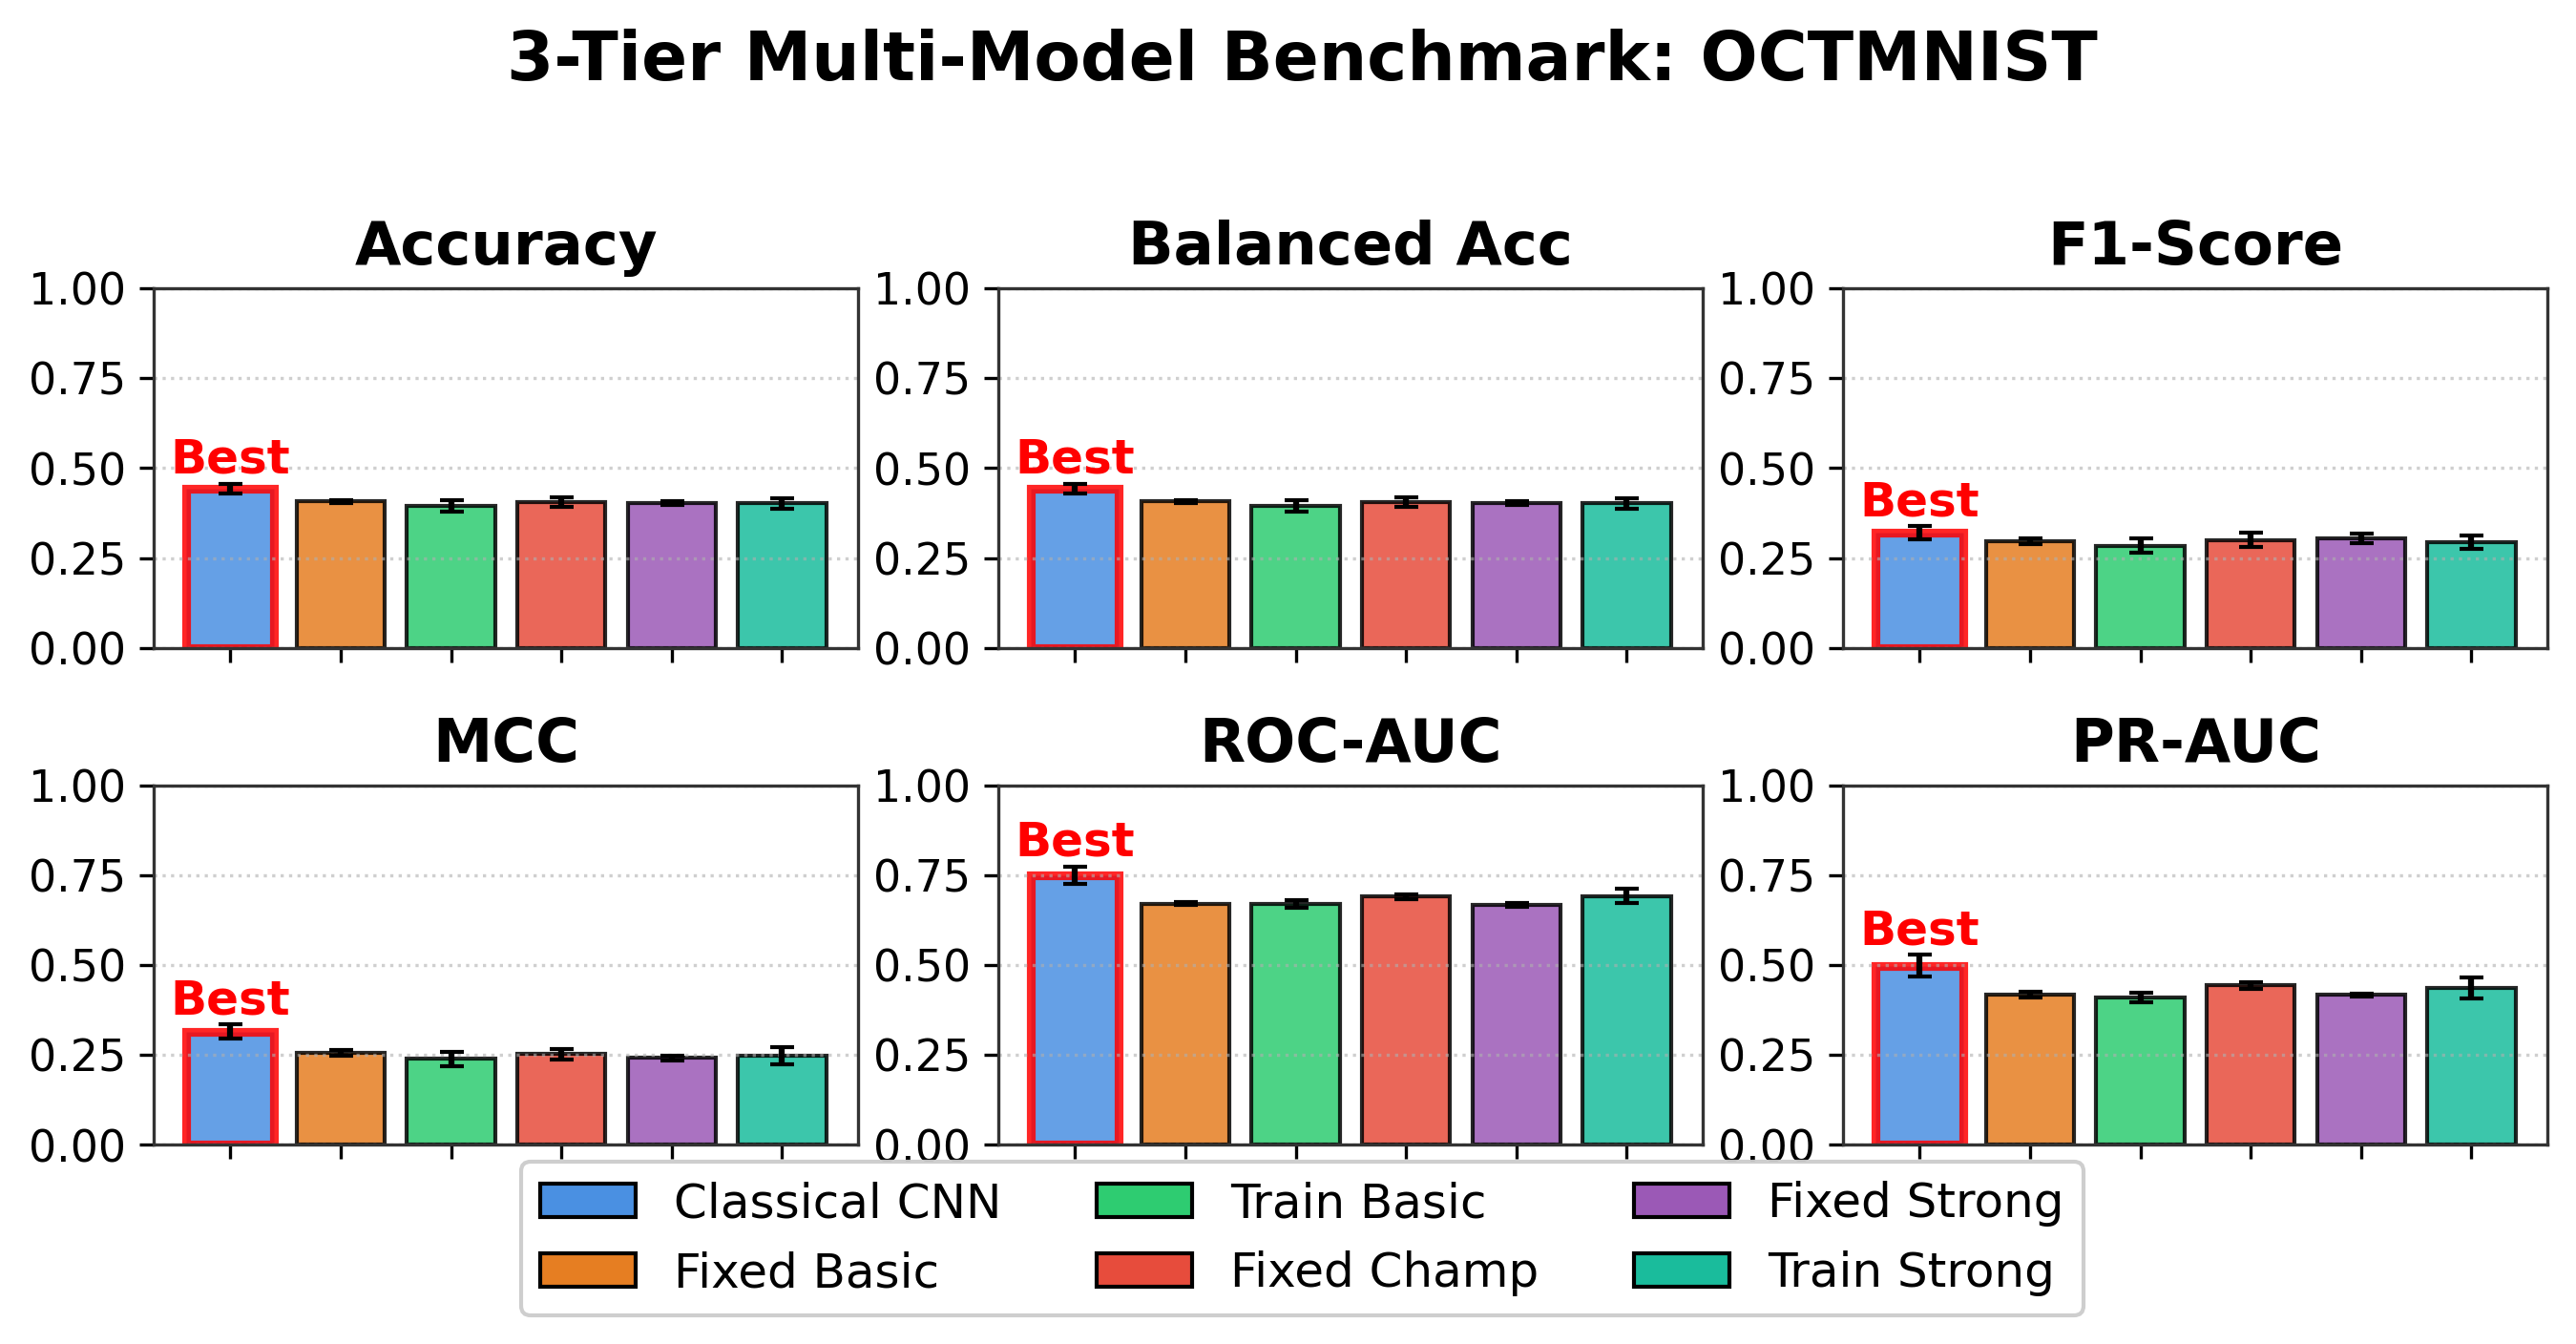
\includegraphics[width=0.78\textwidth]{figures/Fig3_octmnist_benchmark.png}
\caption{Empirical 10-seed performance comparison on OCTMNIST ($L=1$), demonstrating classical CNN dominance and the Tier-3 trainability effect.}
\label{fig:benchmarks_oct}
\end{figure}

\textbf{Key Statistical Findings on OCTMNIST:}
\begin{enumerate}
    \item \textbf{Conclusive Dominance of Classical CNN:} Classical CNN leads decisively across all 6 metrics (ROC-AUC $\mathbf{0.7505 \pm 0.0227}$, PR-AUC $\mathbf{0.4991 \pm 0.0282}$, Acc/BAcc $\mathbf{0.4433 \pm 0.0128}$), outperforming the best quantum model with $p < 0.001$ and huge effect sizes (\textbf{Cohen's $d = +2.108$} for ROC-AUC; \textbf{$d = +1.874$} for BAcc).
    \item \textbf{Tier-3 Trainability Effect:} \texttt{Trainable Strongly} ($0.6922 \pm 0.0189$) significantly surpasses \texttt{Fixed Strongly} ($0.6690 \pm 0.0052$) with $\Delta = +0.0232$ ROC-AUC ($p_{\text{wilcoxon}} = 0.0098 < 0.01$, \textbf{Cohen's $d = +1.050$}).
    \item \textbf{Statistical Tie with Fixed Champion:} \texttt{Trainable Strongly} ($0.6922$) only ties statistically with \texttt{Fixed random\_L1} ($0.6912 \pm 0.0067, \Delta = +0.0010, p = 0.8875$, ns; Cohen's $d = +0.046$).
\end{enumerate}

\subsection{Optimization Dynamics \& Gradient Health}
Analyses of training trajectories (Fig.~\ref{fig:dynamics_convergence} and Fig.~\ref{fig:dynamics_gradients}) confirm:
\begin{itemize}
    \item \textbf{Convergence:} All models reach asymptotic loss plateaus within $12 - 15$ epochs without divergence.
    \item \textbf{Angle Trajectories $\theta(t)$:} Rotational angles smoothly transition from initial states toward localized attractors.
    \item \textbf{Gradient Norms $\|\nabla_\theta \mathcal{L}\|_2$:} For the trainable strongly-entangling ansatz, quantum gradient $L_2$ norms remain within approximately $0.2$--$0.5$ on the seed-averaged curve (individual seeds peaking near $1.3$), well above the vanishing-gradient scale, ruling out barren plateaus in these shallow 4-qubit circuits \cite{mcclean2018barren}.
\end{itemize}

\begin{figure}[t]
\centering
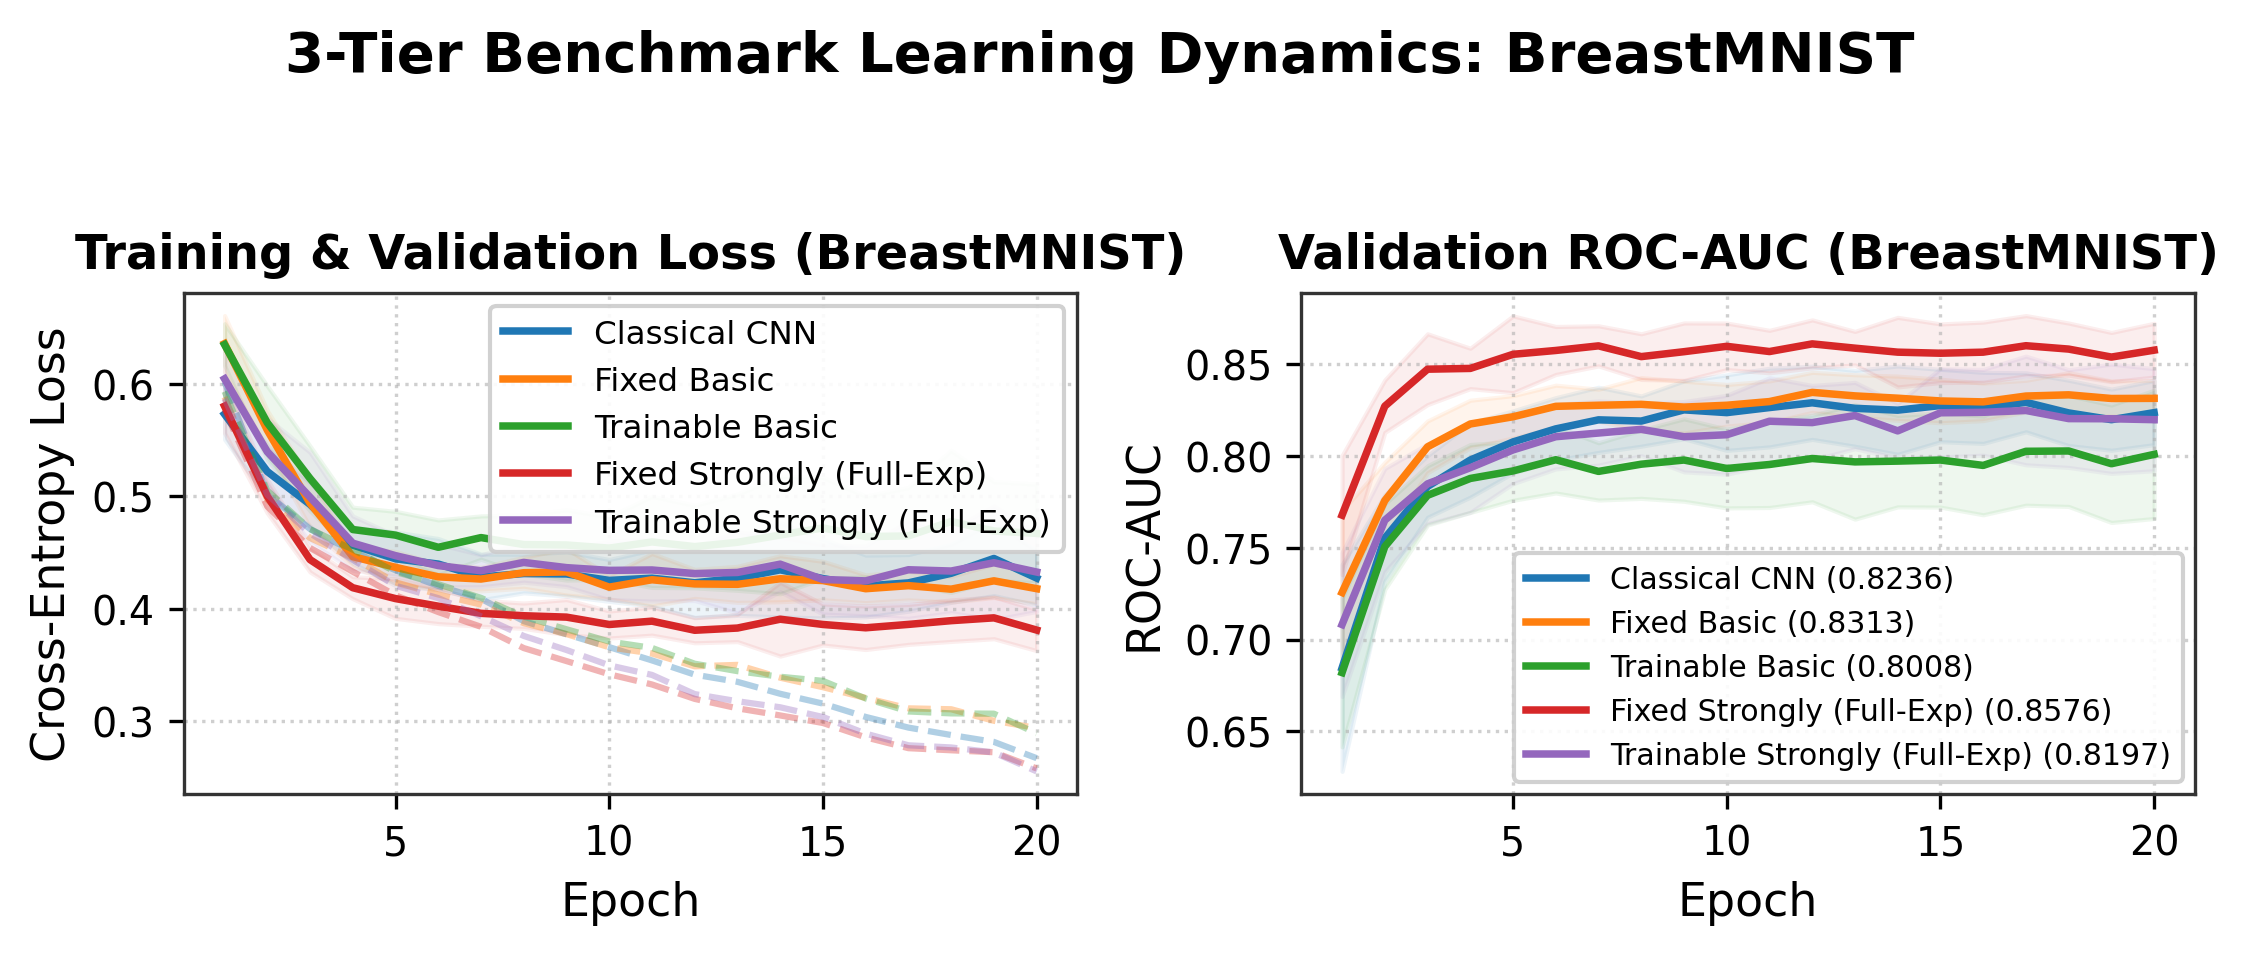
\includegraphics[width=0.46\textwidth]{figures/Fig4a_breastmnist_curves.png}
\hfill
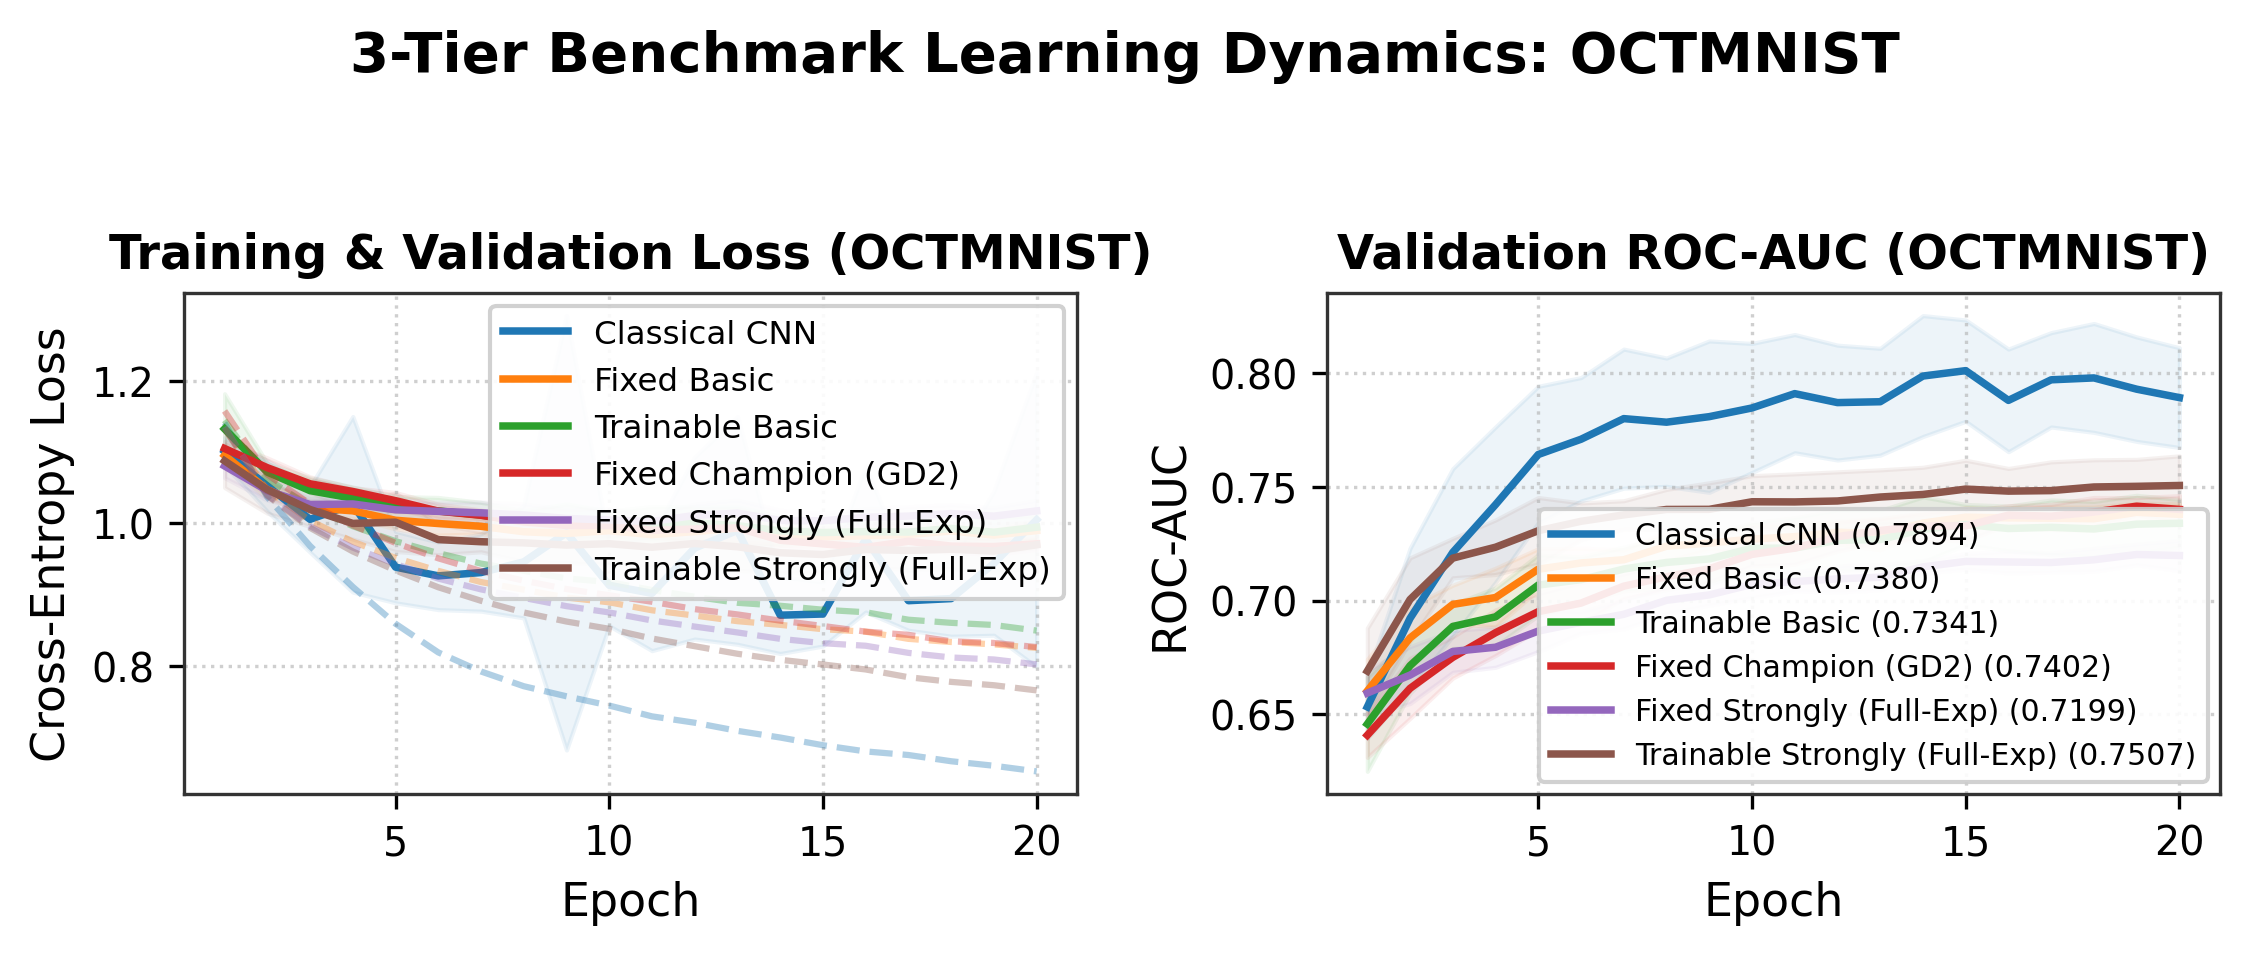
\includegraphics[width=0.46\textwidth]{figures/Fig4b_octmnist_curves.png}
\caption{Training and validation convergence dynamics across 10 seeds: (a) Loss and ROC-AUC convergence on BreastMNIST; (b) Loss and ROC-AUC convergence on OCTMNIST.}
\label{fig:dynamics_convergence}
\end{figure}

\begin{figure}[t]
\centering
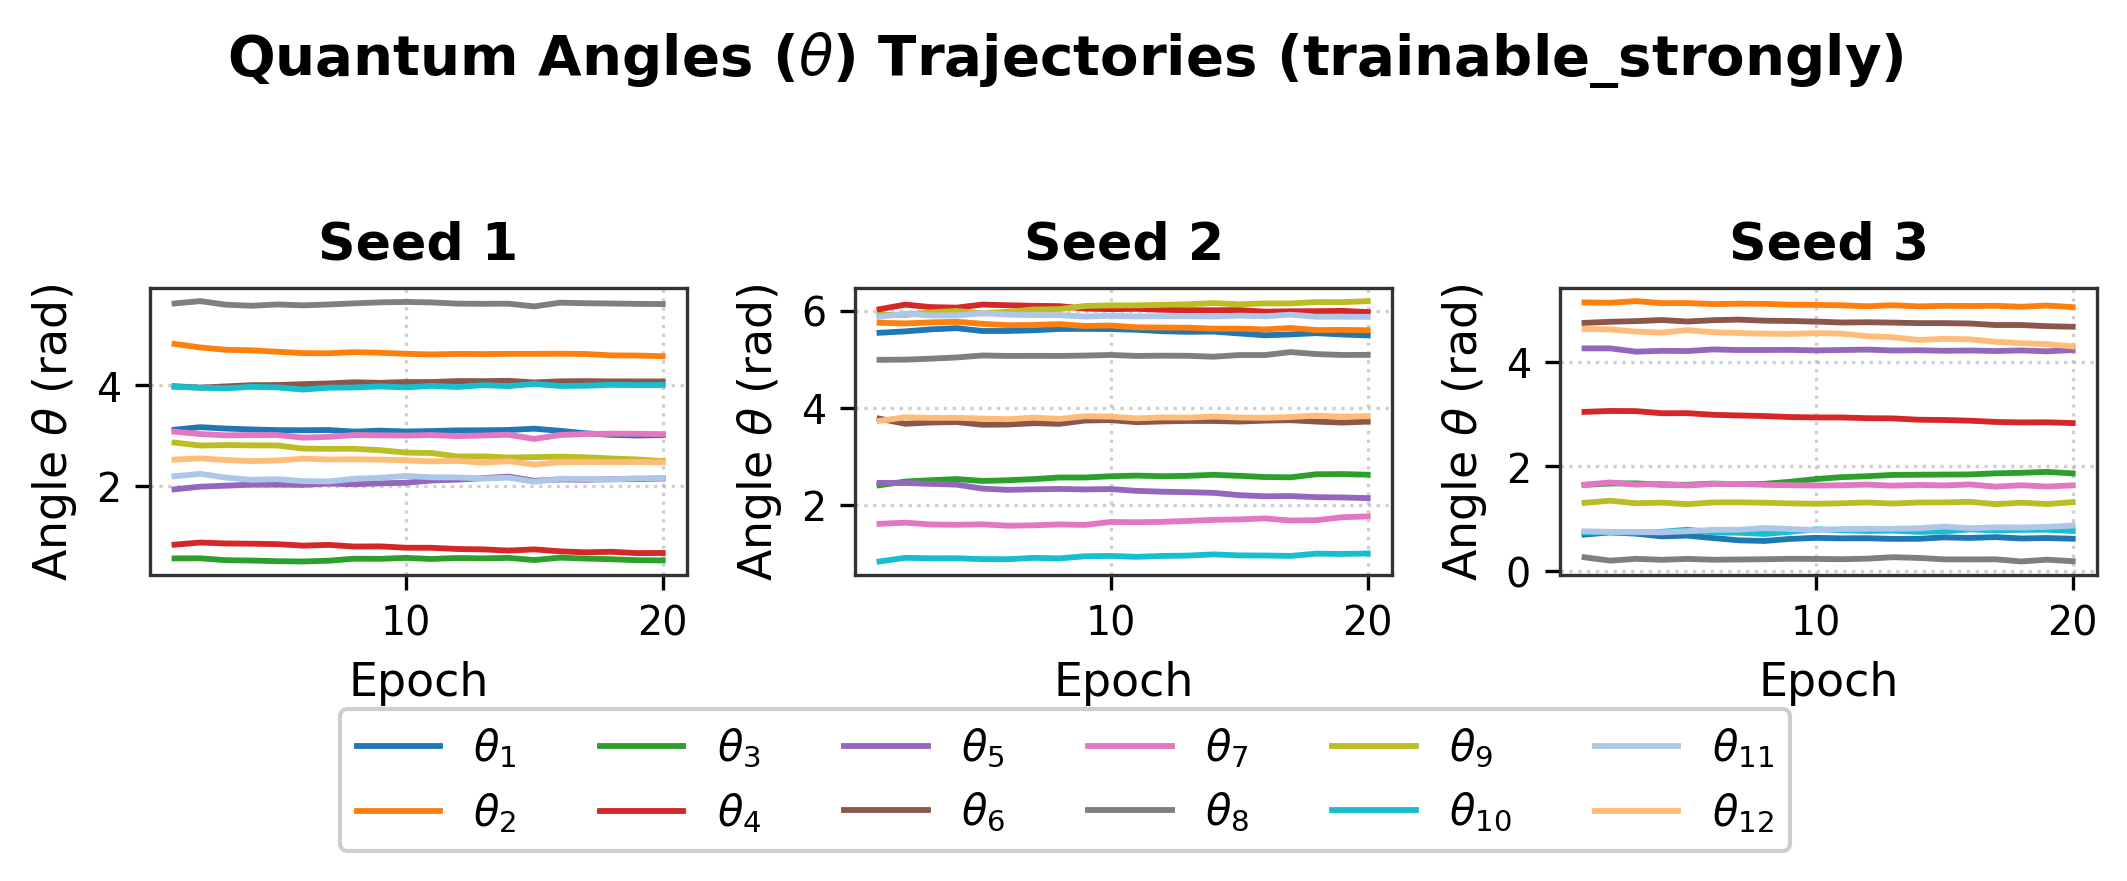
\includegraphics[width=0.46\textwidth]{figures/Fig4c_theta_trajectories.png}
\hfill
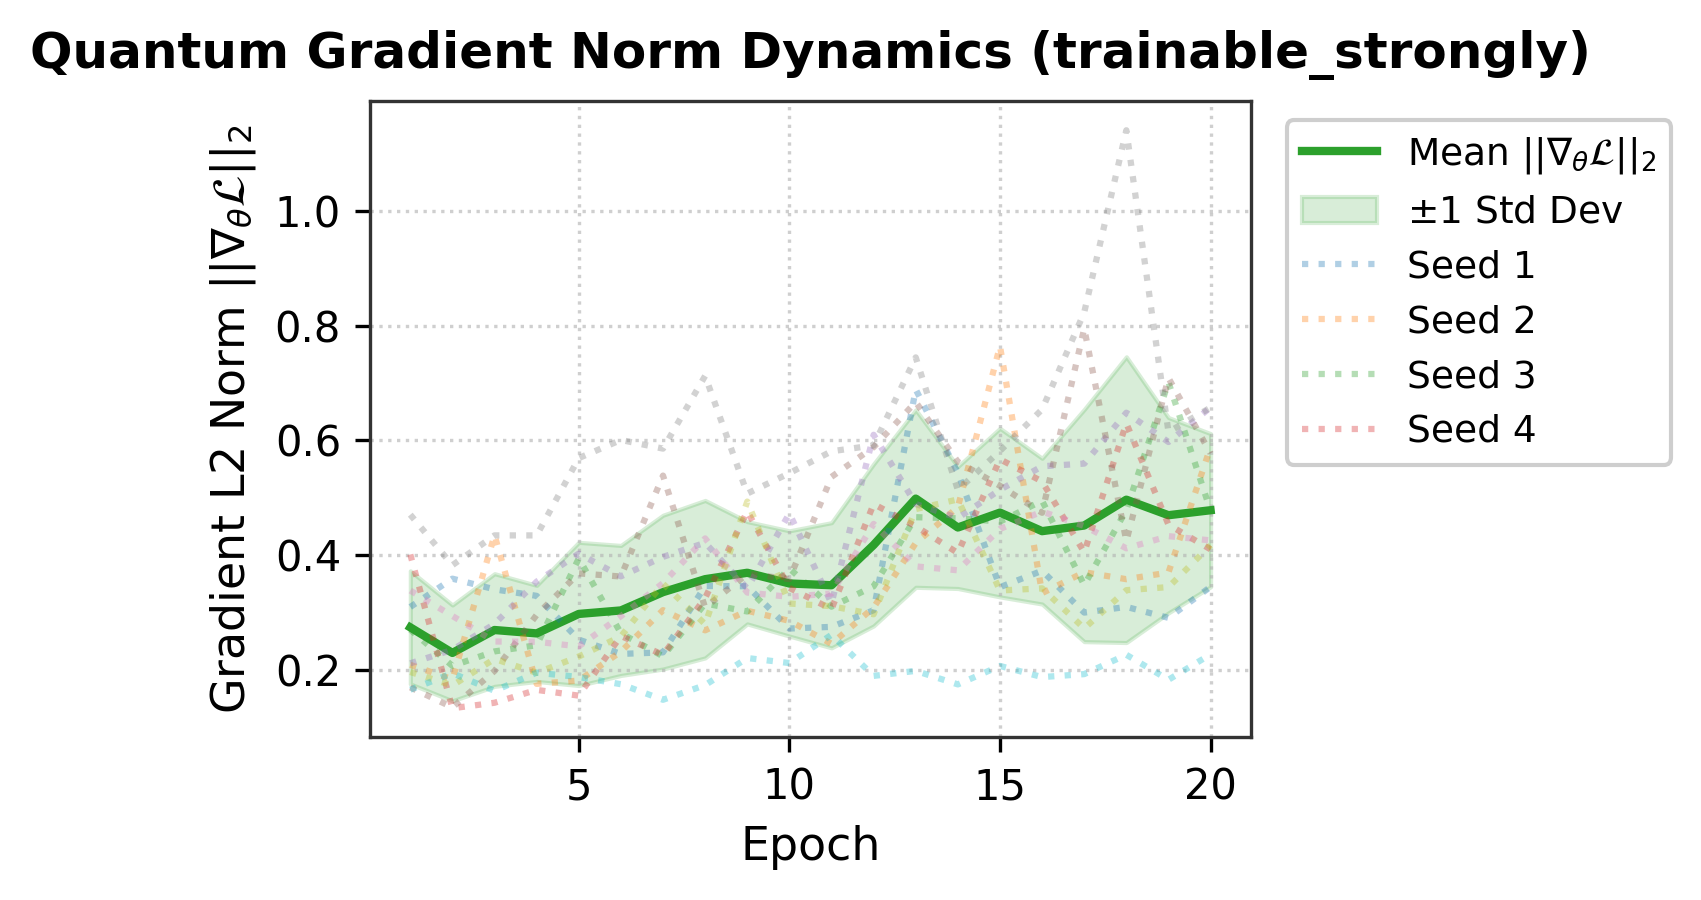
\includegraphics[width=0.46\textwidth]{figures/Fig4d_gradient_norms.png}
\caption{Quantum optimization dynamics: (a) Rotational angle trajectories $\theta(t)$ over 20 epochs; (b) Parameter gradient $L_2$ norms $\|\nabla_\theta \mathcal{L}\|_2$ confirming healthy gradient flow.}
\label{fig:dynamics_gradients}
\end{figure}

\subsection{Computational Latency \& Hardware Costs}
Table~\ref{tab:latency} breaks down CPU inference latency and training wall-clock time.

\begin{table}[t]
\caption{Inference latency and computational cost on Intel CPU.}
\label{tab:latency}
\centering
\small
\resizebox{\textwidth}{!}{%
\begin{tabular}{@{}l l c c c@{}}
\toprule
\textbf{Model} & \textbf{Phase} & \textbf{Mean Latency} & \textbf{Ratio} & \textbf{Kernel Params} \\
\midrule
\textbf{Classical CNN} & Forward Pass & \textbf{$0.310\text{ ms}$} & \textbf{$1.0\times$} & $20$ \\
\midrule
\multirow{3}{*}{\textbf{Fixed Quanv}} & FE ($196$ patches) & $220.187\text{ ms}$ & $710.3\times$ & \textbf{$0$} \\
\addlinespace[2pt]
& Classifier Head & $0.034\text{ ms}$ & $0.11\times$ & Identical \\
\addlinespace[2pt]
& \textbf{End-to-End} & \textbf{$220.221\text{ ms}$} & \textbf{$710.4\times$} & \textbf{$0$} \\
\midrule
\textbf{Trainable Quanv} & \textbf{End-to-End} & \textbf{$\sim 220.25\text{ ms}$} & \textbf{$\sim 710.5\times$} & $12 - 24$ \\
\bottomrule
\end{tabular}%
}
\end{table}

Key computational insights include:
\begin{itemize}
    \item Over $99.98\%$ of execution time is spent on simulating $196$ quantum statevector evolutions on CPU.
    \item Although simulation is $\sim 710\times$ slower than classical convolution, an inference latency of $\approx 0.22\text{ s/image}$ is potentially acceptable for offline screening or low-throughput computer-aided diagnosis workflows.
    \item Fixed quanvolutions allow one-time feature precomputation, reducing 10-seed training time to just $18\text{ seconds}$.
\end{itemize}

\section{Discussion}

\subsection{Decoupling Data Regimes: Capacity Bottleneck vs. Regularization}
The divergent outcomes between BreastMNIST and OCTMNIST highlight a fundamental architectural principle:
\begin{itemize}
    \item \textbf{Small Data Regime (BreastMNIST --- 546 train samples, binary):} Classical convolutions with unconstrained weights readily overfit spurious artifacts. The fixed 4-qubit quantum transformation acts as a rigid \textbf{Structural Regularizer} in Hilbert space, compressing the optimization search space and resulting in a $\sim 2.7\times$ reduction in variance ($0.0090$ vs. $0.0246$) and peak ROC-AUC ($0.8521$).
    \item \textbf{Large Multi-Class Regime (OCTMNIST --- 3,500 train samples, 4 classes):} Separating 4 subtle retinal pathologies requires high spatial feature flexibility. Shallow 4-qubit kernels hit an \textbf{Expressibility Bottleneck}, whereas classical convolutions scale effectively to dominate the task ($0.7505$ vs. $0.6922$).
\end{itemize}

\subsection{Potency of Quantum Inductive Bias in Zero-Parameter Kernels}
A major finding is that zero-parameter fixed quantum circuits (\texttt{Fixed Basic} and \texttt{Fixed Strongly}) achieved top-tier performance on BreastMNIST, outperforming heavily parameterized trainable counterparts. This confirms that adding trainable parameters to the quantum circuit does not guarantee improved generalization in low-data regimes; an appropriately designed fixed circuit already provides sufficient inductive bias.

\subsection{Clinical Relevance in Medical Diagnosis}
In screening scenarios, false negatives are vastly more costly than false positives. Thus, PR-AUC under class imbalance serves as the critical clinical metric. The fact that \texttt{Fixed Strongly Quanvolution} reaches a PR-AUC of $\mathbf{0.9182 \pm 0.0067}$ ($d = +1.332$ over Classical CNN at $0.9041$) demonstrates the unique sensitivity of quantum kernel representations in isolating rare pathological cases.

\section{Threats to Validity \& Limitations}
We explicitly note four methodological boundaries of this benchmark:
\begin{enumerate}
    \item \textbf{Resolution and Patch Constraints:} This study evaluates $28 \times 28$ MedMNIST images partitioned into local $2 \times 2$ patches ($4$ qubits). Scaling to standard clinical resolutions ($224 \times 224$ or $512 \times 512$) will require multi-scale patch decomposition or hierarchical pooling to avoid combinatorial simulation bottlenecks.
    \item \textbf{Subsampled Dataset Scale:} While BreastMNIST evaluates the full benchmark ($780$ images), the OCTMNIST experiment utilizes a balanced subset of $5{,}000$ images from the complete $\approx 97{,}000$ collection to enable extensive 10-seed ablation. Future benchmarks should assess behavior under full-scale multi-class distributions.
    \item \textbf{Noiseless Statevector Simulation:} All quantum transformations were executed using exact statevector simulation (\texttt{default.qubit}). Physical NISQ QPU deployment will inevitably introduce gate infidelities, readout noise, and qubit crosstalk, which may degrade subtle quantum inductive biases.
    \item \textbf{Exploratory Multiple Comparisons:} Given the evaluation of $6$ metrics across $2$ datasets, the statistical tests serve as exploratory indicators of relative model behavior rather than confirmatory clinical trial endpoints.
\end{enumerate}

\section{Conclusion \& Future Work}
This study presented a rigorous, symmetrical benchmark comparing Trainable and Fixed Quanvolutions against a Classical CNN on MedMNIST.

We summarize three primary conclusions:
\begin{enumerate}
    \item \textbf{Quantum advantage is strictly data-regime dependent:} Quanvolution provides significant ranking and stability advantages on small, imbalanced datasets, but classical CNNs decisively dominate on larger multi-class benchmarks.
    \item \textbf{Zero-parameter fixed kernels provide powerful inductive bias:} Fixed circuits deliver superior variance stability ($\sim 2.7\times$ lower std) and top PR-AUC without training kernel parameters.
    \item \textbf{Trainability is localized:} Optimizing quantum rotational angles yields gains only within the same circuit family, failing to outperform optimal fixed baselines.
\end{enumerate}

\textbf{Future Work:} We plan to integrate GPU-accelerated tensor network backends (e.g., NVIDIA cuQuantum) to evaluate noise resilience under realistic NISQ hardware models.

\begin{thebibliography}{99}
\bibitem{litjens2017survey} Litjens, G., et al.: A survey on deep learning in medical image analysis. Medical Image Analysis \textbf{42}, 60--88 (2017)
\bibitem{yang2023medmnist} Yang, J., et al.: MedMNIST v2 - A large-scale lightweight benchmark for 2D and 3D biomedical image classification. Scientific Data \textbf{10}(1), 41 (2023)
\bibitem{esteva2019guide} Esteva, A., et al.: A guide to deep learning in healthcare. Nature Medicine \textbf{25}(1), 24--29 (2019)
\bibitem{shorten2019survey} Shorten, C., Khoshgoftaar, T.M.: A survey on image data augmentation for deep learning. J. Big Data \textbf{6}(1), 60 (2019)
\bibitem{biamonte2017quantum} Biamonte, J., et al.: Quantum machine learning. Nature \textbf{549}(7671), 195--202 (2017)
\bibitem{cerezo2021variational} Cerezo, M., et al.: Variational quantum algorithms. Nature Reviews Physics \textbf{3}(9), 625--644 (2021)
\bibitem{henderson2020quanvolutional} Henderson, M., Shakya, S., Pradhan, S., Cook, T.: Quanvolutional neural networks: powering image recognition with quantum circuits. Quantum Machine Intelligence \textbf{2}(1), 2 (2020)
\bibitem{huang2021power} Huang, H.Y., et al.: Power of data in quantum machine learning. Nature Communications \textbf{12}(1), 2631 (2021)
\bibitem{vu2024exploring} Vu, T.H., Le, H.L., Pham, T.B.: Exploring the features of quanvolutional neural networks for improved image classification. Quantum Machine Intelligence \textbf{6}(1), 15 (2024)
\bibitem{altares2021automatic} Altares-L{\'o}pez, F.M., Ribeiro, A., Garc{\'i}a-Ripoll, J.J.: Automatic design of quantum feature maps. Quantum Science and Technology \textbf{6}(4), 045015 (2021)
\bibitem{azevedo2022quantum} Azevedo, F.S., Silva, A., Oliveira, I.C.: Quantum transfer learning for breast cancer detection. Quantum Information Processing \textbf{21}(3), 112 (2022)
\bibitem{hoang2023efficient} Hoang, Q.N., Pham, T.T., Dang, D.N.M.: Efficient hybrid quantum-classical convolutional neural network with feature propagation layer for multi-class image classification. In: Proc. Int. Conf. Adv. Eng. Theory Appl. (AETA), pp. 1--10 (2023)
\bibitem{kubler2021inductive} K{\"u}bler, J., Buchholz, S., Sch{\"o}lkopf, B.: The inductive bias of quantum kernels. In: Advances in Neural Information Processing Systems (NeurIPS), vol. 34, pp. 12661--12673 (2021)
\bibitem{cong2019quantum} Cong, I., Choi, S., Lukin, M.D.: Quantum convolutional neural networks. Nature Physics \textbf{15}(12), 1273--1278 (2019)
\bibitem{bergholm2018pennylane} Bergholm, V., et al.: PennyLane: Automatic differentiation of quantum machine learning circuits. arXiv:1811.04968 (2018)
\bibitem{schuld2019evaluating} Schuld, M., Bergholm, V., Gogolin, C., Izaac, J., Killoran, N.: Evaluating analytic gradients on quantum hardware. Physical Review A \textbf{99}(3), 032331 (2019)
\bibitem{mcclean2018barren} McClean, J.R., Boixo, S., Smelyanskiy, V.N., Babbush, R., Neven, H.: Barren plateaus in quantum neural network training landscapes. Nature Communications \textbf{9}(1), 4812 (2018)
\bibitem{sannakki2026medmnist} Sannakki, S.S., Rajpurohit, V.S., Kulkarni, V.B.: Benchmarking medical image classification with variational quantum circuits on NISQ hardware. Scientific Reports \textbf{16}(1), 1042 (2026)
\bibitem{schuld2024needqml} Schuld, M., Killoran, N.: Is quantum machine learning really classical with extra steps? A critical empirical assessment. Quantum Machine Intelligence \textbf{6}(2), 42 (2024)
\end{thebibliography}

\end{document}
